%% LyX 2.2.0 created this file.  For more info, see http://www.lyx.org/.
%% Do not edit unless you really know what you are doing.
\documentclass[english]{article}
\usepackage[T1]{fontenc}
\usepackage[latin9]{inputenc}
\usepackage[letterpaper]{geometry}
\geometry{verbose,tmargin=3cm,bmargin=3cm,lmargin=2cm,rmargin=2cm}
\setlength{\parindent}{0bp}
\usepackage{babel}
\usepackage{amsmath}
\usepackage{amsthm}
\usepackage{amssymb}
\usepackage{graphicx}
\usepackage{setspace}
\onehalfspacing
\usepackage[unicode=true,pdfusetitle,
 bookmarks=true,bookmarksnumbered=true,bookmarksopen=true,bookmarksopenlevel=3,
 breaklinks=false,pdfborder={0 0 1},backref=false,colorlinks=false]
 {hyperref}

\makeatletter

%%%%%%%%%%%%%%%%%%%%%%%%%%%%%% LyX specific LaTeX commands.
%% Because html converters don't know tabularnewline
\providecommand{\tabularnewline}{\\}

\makeatother

\begin{document}

\title{Nonparametric Estimation of IV Model}

\author{Jiaqi Yin}
\maketitle

\section{Estimations}

We consider binary instrumental variable model Fig.(\ref{fig:Directed-acyclic-graph})
, where we have $A\perp U$, $C\perp A\mid(B,U)$ and $A$ is not
independent of $B$. We have $A,B,C\in\left\{ 0,1\right\} $. Let
$P_{cb\cdot a}=Pr(C=c,B=b\mid A=a)$. Sufficient and necessary conditions
for IV model are
\begin{equation}
\begin{cases}
P_{00\cdot0}+ & P_{10\cdot1}\leq1\\
P_{01\cdot0}+ & P_{11\cdot1}\leq1\\
P_{10\cdot0}+ & P_{00\cdot1}\leq1\\
P_{11\cdot0}+ & P_{01\cdot1}\leq1
\end{cases}.\label{eq:iv-inqua}
\end{equation}

Ineq.(\ref{eq:iv-inqua}) are also called IV-inequalites. 

\begin{figure}
\begin{centering}
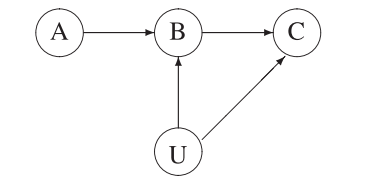
\includegraphics[bb = 0 0 200 100, draft, type=eps]{C:/Users/Jacky/Dropbox/research/iv_model/iv_model.PNG}
\par\end{centering}
\caption{Directed acyclic graph which represents the instrumental variable
model.\label{fig:Directed-acyclic-graph}}
\end{figure}

Suppose our sample size is $n$, and each individual is i.i.d. Let
$n_{cba}=\sum_{i=1}^{n}\mathbb{I}\left\{ A=a,B=b,C=c\right\} .$ We
need to esitimate $P_{cb\cdot a}$. The log-likelihood is 
\[
l(P_{cb\cdot a})=\sum_{a,b,c}n_{cba}\log P_{cb\cdot a}.
\]

Of cousse, we assume $P_{cb\cdot a}>0$. An optimization question
is raised as follows, 
\[
\begin{cases}
\min & -\sum_{a,b,c}n_{cba}\log P_{cb\cdot a}\\
\text{subject to} & P_{00\cdot0}+P_{10\cdot1}\leq1\\
 & P_{01\cdot0}+P_{11\cdot1}\leq1\\
 & P_{10\cdot0}+P_{00\cdot1}\leq1\\
 & P_{11\cdot0}+P_{01\cdot1}\leq1\\
 & P_{00\cdot0}+P_{01\cdot0}+P_{10\cdot0}+P_{11\cdot0}=1\\
 & P_{00\cdot1}+P_{01\cdot1}+P_{10\cdot1}+P_{11\cdot1}=1
\end{cases},
\]
where objective function and feasible set are convex. The Lagrange
fucntion is 
\begin{align*}
L(P_{abc},\lambda,\nu) & =-\sum_{a,b,c}n_{cba}\log P_{cb\cdot a}+\lambda_{1}\left(P_{00\cdot0}+P_{10\cdot1}-1\right)+\lambda_{2}\left(P_{01\cdot0}+P_{11\cdot1}-1\right)\\
 & \quad+\lambda_{3}\left(P_{10\cdot0}+P_{00\cdot1}-1\right)+\lambda_{4}\left(P_{11\cdot0}+P_{01\cdot1}-1\right)\\
 & \quad+\nu_{1}\left(P_{00\cdot0}+P_{01\cdot0}+P_{10\cdot0}+P_{11\cdot0}-1\right)+\nu_{2}\left(P_{00\cdot1}+P_{01\cdot1}+P_{10\cdot1}+P_{11\cdot1}-1\right).
\end{align*}

Becasue Slater's condition is satisfied, strong duality holds. Let
$p_{cb\cdot a}^{*}$ and $\left(\lambda^{*},\nu^{*}\right)$ be primal
and dual optimal points. We further have KKT conditions,

\[
\begin{cases}
p_{00\cdot0}^{*}+p_{10\cdot1}^{*}-1\leq0\\
p_{01\cdot0}^{*}+p_{11\cdot1}^{*}-1\leq0\\
p_{10\cdot0}^{*}+p_{00\cdot1}^{*}-1\leq0\\
p_{11\cdot0}^{*}+p_{01\cdot1}^{*}-1\leq0\\
p_{00\cdot0}^{*}+p_{01\cdot0}^{*}+p_{10\cdot0}^{*}+p_{11\cdot0}^{*}-1=0\\
p_{00\cdot1}^{*}+p_{01\cdot1}^{*}+p_{10\cdot1}^{*}+p_{11\cdot1}^{*}-1=0\\
\lambda_{i}^{*}\ge0,\quad i=1,2,3,4\\
\lambda_{1}^{*}\left(p_{00\cdot0}^{*}+p_{10\cdot1}^{*}-1\right)=0\\
\lambda_{2}^{*}\left(p_{01\cdot0}^{*}+p_{11\cdot1}^{*}-1\right)=0\\
\lambda_{3}^{*}\left(p_{10\cdot0}^{*}+p_{00\cdot1}^{*}-1\right)=0\\
\lambda_{4}^{*}\left(p_{11\cdot0}^{*}+p_{01\cdot1}^{*}-1\right)=0\\
-\frac{n_{000}}{p_{00\cdot0}^{*}}+\lambda_{1}^{*}+\nu_{1}^{*}=0;\quad-\frac{n_{101}}{p_{10\cdot1}^{*}}+\lambda_{1}^{*}+\nu_{2}^{*}=0;\\
-\frac{n_{010}}{p_{01\cdot0}^{*}}+\lambda_{2}^{*}+\nu_{1}^{*}=0;\quad-\frac{n_{111}}{p_{11\cdot1}^{*}}+\lambda_{2}^{*}+\nu_{2}^{*}=0;\\
-\frac{n_{100}}{p_{10\cdot0}^{*}}+\lambda_{3}^{*}+\nu_{1}^{*}=0;\quad-\frac{n_{001}}{p_{00\cdot1}^{*}}+\lambda_{3}^{*}+\nu_{2}^{*}=0;\\
-\frac{n_{110}}{p_{11\cdot0}^{*}}+\lambda_{4}^{*}+\nu_{1}^{*}=0;\quad-\frac{n_{011}}{p_{01\cdot1}^{*}}+\lambda_{4}^{*}+\nu_{2}^{*}=0.
\end{cases}
\]

We start by noting that $\lambda^{*}$act as slack variables in the
last four equations, so it can be eliminated, leaving

\[
\begin{cases}
p_{00\cdot0}^{*}+p_{10\cdot1}^{*}-1\leq0\\
p_{01\cdot0}^{*}+p_{11\cdot1}^{*}-1\leq0\\
p_{10\cdot0}^{*}+p_{00\cdot1}^{*}-1\leq0\\
p_{11\cdot0}^{*}+p_{01\cdot1}^{*}-1\leq0\\
p_{00\cdot0}^{*}+p_{01\cdot0}^{*}+p_{10\cdot0}^{*}+p_{11\cdot0}^{*}-1=0\\
p_{00\cdot1}^{*}+p_{01\cdot1}^{*}+p_{10\cdot1}^{*}+p_{11\cdot1}^{*}-1=0\\
\left(\frac{n_{000}}{p_{00\cdot0}^{*}}-\nu_{1}^{*}\right)\left(p_{00\cdot0}^{*}+p_{10\cdot1}^{*}-1\right)=0;\quad\left(\frac{n_{101}}{p_{10\cdot1}^{*}}-\nu_{2}^{*}\right)\left(p_{00\cdot0}^{*}+p_{10\cdot1}^{*}-1\right)=0\\
\left(\frac{n_{010}}{p_{01\cdot0}^{*}}-\nu_{1}^{*}\right)\left(p_{01\cdot0}^{*}+p_{11\cdot1}^{*}-1\right)=0;\quad\left(\frac{n_{111}}{p_{11\cdot1}^{*}}-\nu_{2}^{*}\right)\left(p_{01\cdot0}^{*}+p_{11\cdot1}^{*}-1\right)=0\\
\left(\frac{n_{100}}{p_{10\cdot0}^{*}}-\nu_{1}^{*}\right)\left(p_{10\cdot0}^{*}+p_{00\cdot1}^{*}-1\right)=0;\quad\left(\frac{n_{001}}{p_{00\cdot1}^{*}}-\nu_{2}^{*}\right)\left(p_{10\cdot0}^{*}+p_{00\cdot1}^{*}-1\right)=0\\
\left(\frac{n_{110}}{p_{11\cdot0}^{*}}-\nu_{1}^{*}\right)\left(p_{11\cdot0}^{*}+p_{01\cdot1}^{*}-1\right)=0;\quad\left(\frac{n_{011}}{p_{01\cdot1}^{*}}-\nu_{2}^{*}\right)\left(p_{11\cdot0}^{*}+p_{01\cdot1}^{*}-1\right)=0\\
\nu_{1}^{*}\leq\min\left\{ \frac{n_{000}}{p_{00\cdot0}^{*}},\frac{n_{010}}{p_{01\cdot0}^{*}},\frac{n_{100}}{p_{10\cdot0}^{*}},\frac{n_{110}}{p_{11\cdot0}^{*}}\right\} \\
\nu_{2}^{*}\leq\min\left\{ \frac{n_{101}}{p_{10\cdot1}^{*}},\frac{n_{111}}{p_{11\cdot1}^{*}},\frac{n_{001}}{p_{00\cdot1}^{*}},\frac{n_{011}}{p_{01\cdot1}^{*}}\right\} 
\end{cases}.
\]
If $p_{00\cdot0}^{*}+p_{10\cdot1}^{*}-1<0;p_{01\cdot0}^{*}+p_{11\cdot1}^{*}-1<0;p_{10\cdot0}^{*}+p_{00\cdot1}^{*}-1<0;p_{11\cdot0}^{*}+p_{01\cdot1}^{*}-1<0$,
we will have 
\begin{align*}
\nu_{1}^{*} & =\frac{n_{000}}{p_{00\cdot0}^{*}}=\frac{n_{010}}{p_{01\cdot0}^{*}}=\frac{n_{100}}{p_{10\cdot0}^{*}}=\frac{n_{110}}{p_{11\cdot0}^{*}},\\
\nu_{2}^{*} & =\frac{n_{101}}{p_{10\cdot1}^{*}}=\frac{n_{111}}{p_{11\cdot1}^{*}}=\frac{n_{001}}{p_{00\cdot1}^{*}}=\frac{n_{011}}{p_{01\cdot1}^{*}}.
\end{align*}
Further, $\nu_{1}^{*}=n_{0}$, $\nu_{2}^{*}=n_{1}$, and $p_{cb\cdot a}^{*}=\frac{n_{cba}}{n_{a}}$.

However, once we consider sampling variability, we could have the
case such that $\frac{n_{cba}}{n_{a}}+\frac{n_{(1-c)b(1-a)}}{n_{1-a}}>1$,
which voilates IV Inqualities if we estimate $p_{cb\cdot a}^{*}=\frac{n_{cba}}{n_{a}}.$
When we have such case, let $p_{c'b'\cdot a'}^{*}+p_{(1-c')b'\cdot(1-a')}^{*}=1$
for some $a',b',c'$. Consider nonzero $p_{cb\cdot a}^{*}$ and $\sum_{bc}p_{cb\cdot a}^{*}=1$,
we could not have $p_{(1-c')b'\cdot a'}^{*}+p_{c'b'\cdot(1-a')}^{*}=1$,
$p_{(1-c')(1-b')\cdot a'}^{*}+p_{c'(1-b')\cdot(1-a')}^{*}=1$ or $p_{c'(1-b')\cdot a'}^{*}+p_{(1-c')(1-b')\cdot(1-a')}^{*}=1$
(once any one of it holds, we will have zero proabability). WOLG,
let $c'=0,b'=0,a'=0$, and $\frac{n_{000}}{n_{0}}+\frac{n_{101}}{n_{1}}>1$.
Let $p_{00\cdot0}^{*}+p_{10\cdot1}^{*}=1$, $p_{01\cdot0}^{*}+p_{11\cdot1}^{*}<1$,
$p_{10\cdot0}^{*}+p_{00\cdot1}^{*}<1$, and $p_{11\cdot0}^{*}+p_{01\cdot1}^{*}<1$. 

Further, 
\begin{align}
\frac{n_{010}}{p_{01\cdot0}^{*}}=\frac{n_{100}}{p_{10\cdot0}^{*}}=\frac{n_{110}}{p_{11\cdot0}^{*}}=\nu_{1}^{*} & <\frac{n_{000}}{p_{00\cdot0}^{*}}\label{eq:nu1}\\
\frac{n_{111}}{p_{11\cdot1}^{*}}=\frac{n_{001}}{p_{00\cdot1}^{*}}=\frac{n_{011}}{p_{01\cdot1}^{*}}=\nu_{2}^{*} & <\frac{n_{101}}{p_{10\cdot1}^{*}}.\nonumber 
\end{align}

The constraints are updated as 

\begin{equation}
\begin{cases}
p_{00\cdot0}^{*}+p_{10\cdot1}^{*}=1\\
p_{01\cdot0}^{*}+p_{11\cdot1}^{*}+p_{10\cdot0}^{*}+p_{00\cdot1}^{*}+p_{11\cdot0}^{*}+p_{01\cdot1}^{*}=1\\
\frac{n_{010}}{p_{01\cdot0}^{*}}=\frac{n_{100}}{p_{10\cdot0}^{*}}=\frac{n_{110}}{p_{11\cdot0}^{*}}=\nu_{1}^{*}<\frac{n_{000}}{p_{00\cdot0}^{*}}\\
\frac{n_{111}}{p_{11\cdot1}^{*}}=\frac{n_{001}}{p_{00\cdot1}^{*}}=\frac{n_{011}}{p_{01\cdot1}^{*}}=\nu_{2}^{*}<\frac{n_{101}}{p_{10\cdot1}^{*}}\\
p_{01\cdot0}^{*}+p_{10\cdot0}^{*}+p_{11\cdot0}^{*}<1\\
p_{01\cdot1}^{*}+p_{10\cdot1}^{*}+p_{11\cdot1}^{*}<1
\end{cases}.\label{eq:constraints}
\end{equation}

From Eq.(\ref{eq:constraints})-1,2, we have $p_{00\cdot0}^{*}=1-p_{10\cdot1}^{*}=p_{00\cdot1}^{*}+p_{11\cdot0}^{*}+p_{01\cdot1}^{*}$,
and $p_{10\cdot1}^{*}=1-p_{00\cdot0}^{*}=p_{01\cdot0}^{*}+p_{11\cdot1}^{*}+p_{10\cdot0}^{*}$.
Plug them into (\ref{eq:constraints})-3,4, we further have 
\begin{align}
\frac{n_{010}}{p_{01\cdot0}^{*}} & =\frac{n_{100}}{p_{10\cdot0}^{*}}=\frac{n_{110}}{p_{11\cdot0}^{*}}=\frac{n_{0}-n_{000}}{1-p_{00\cdot0}^{*}}=\frac{n_{0}-n_{000}}{p_{10\cdot1}^{*}}.\label{eq:p0s}\\
\frac{n_{111}}{p_{11\cdot1}^{*}} & =\frac{n_{001}}{p_{00\cdot1}^{*}}=\frac{n_{011}}{p_{01\cdot1}^{*}}=\frac{n_{1}-n_{101}}{1-p_{10\cdot1}^{*}}=\frac{n_{1}-n_{101}}{p_{00\cdot0}^{*}}.
\end{align}
From above equations, it yelds 
\begin{align}
p_{01\cdot0}^{*} & =\frac{n_{010}}{n_{0}-n_{000}}p_{10\cdot1}^{*},\quad p_{10\cdot0}^{*}=\frac{n_{100}}{n_{0}-n_{000}}p_{10\cdot1}^{*},\quad p_{11\cdot0}^{*}=\frac{n_{110}}{n_{0}-n_{000}}p_{10\cdot1}^{*};\label{eq:p0}\\
p_{11\cdot1}^{*} & =\frac{n_{111}}{n_{1}-n_{101}}p_{00\cdot0}^{*},\quad p_{00\cdot1}^{*}=\frac{n_{001}}{n_{1}-n_{101}}p_{00\cdot0}^{*},\quad p_{01\cdot1}^{*}=\frac{n_{011}}{n_{1}-n_{101}}p_{00\cdot0}^{*}.\label{eq:p1}
\end{align}
From Ineq.(\ref{eq:constraints})-3,4,5,6, we further have 
\[
\begin{cases}
\frac{n_{0}-n_{000}}{1-p_{00\cdot0}^{*}}<\frac{n_{000}}{p_{00\cdot0}^{*}}\\
\frac{n_{1}-n_{101}}{1-p_{10\cdot1}^{*}}<\frac{n_{101}}{p_{10\cdot1}^{*}}\\
\left(\frac{n_{010}}{n_{0}-n_{000}}+\frac{n_{100}}{n_{0}-n_{000}}+\frac{n_{110}}{n_{0}-n_{000}}\right)p_{10\cdot1}^{*}<1\\
\left(\frac{n_{111}}{n_{1}-n_{101}}+\frac{n_{001}}{n_{1}-n_{101}}+\frac{n_{011}}{n_{1}-n_{101}}\right)p_{00\cdot0}^{*}<1
\end{cases}.
\]
Finally, we have 
\begin{equation}
\max\left\{ 0,1-\frac{n_{101}}{n_{1}}\right\} <p_{00\cdot0}^{*}<\min\left\{ \frac{n_{000}}{n_{0}},1\right\} \label{eq:final constraints}
\end{equation}

Next, we need to maximize $l(p_{cb\cdot a}^{*})=\sum_{a,b,c}n_{cba}\log p_{cb\cdot a}^{*}$,
and we further plug Eq.(\ref{eq:p0})(\ref{eq:p1}) into the log-likelihood

\begin{align*}
l(p_{00\cdot0}^{*}) & =\sum_{a,b,c}n_{cba}\log p_{cb\cdot a}^{*}\\
 & =n_{101}\log p_{10\cdot1}^{*}+n_{010}\log\left(\frac{n_{010}}{n_{0}-n_{000}}p_{10\cdot1}^{*}\right)+n_{100}\log\left(\frac{n_{100}}{n_{0}-n_{000}}p_{10\cdot1}^{*}\right)+n_{110}\log\left(\frac{n_{110}}{n_{0}-n_{000}}p_{10\cdot1}^{*}\right)\\
 & \quad+n_{000}\log p_{00\cdot0}^{*}+n_{111}\log\left(\frac{n_{111}}{n_{1}-n_{101}}p_{00\cdot0}^{*}\right)+n_{001}\log\left(\frac{n_{001}}{n_{1}-n_{101}}p_{00\cdot0}^{*}\right)+n_{011}\log\left(\frac{n_{011}}{n_{1}-n_{101}}p_{00\cdot0}^{*}\right)\\
 & =\left(n_{101}+n_{010}+n_{100}+n_{110}\right)\log\left(1-p_{00\cdot0}^{*}\right)+n_{010}\log\left(\frac{n_{010}}{n_{0}-n_{000}}\right)+n_{100}\log\left(\frac{n_{100}}{n_{0}-n_{000}}\right)+n_{110}\log\left(\frac{n_{110}}{n_{0}-n_{000}}\right)\\
 & \quad+\left(n_{000}+n_{111}+n_{001}+n_{011}\right)\log p_{00\cdot0}^{*}+n_{111}\log\left(\frac{n_{111}}{n_{1}-n_{101}}\right)+n_{001}\log\left(\frac{n_{001}}{n_{1}-n_{101}}\right)+n_{011}\log\left(\frac{n_{011}}{n_{1}-n_{101}}\right)
\end{align*}
The derivative of $l(p_{00\cdot0}^{*})$ is 
\[
l^{'}(p_{00\cdot0}^{*})=\frac{n_{000}+n_{111}+n_{001}+n_{011}}{p_{00\cdot0}^{*}}-\frac{n_{101}+n_{010}+n_{100}+n_{110}}{1-p_{10\cdot0}^{*}}.
\]

Let $l^{'}(p_{00\cdot0}^{*})=0$, we have maximizer $\tilde{p}_{00\cdot0}=\frac{n_{000}+n_{111}+n_{001}+n_{011}}{n}$.
When $p_{00\cdot0}^{*}<\tilde{p}_{00\cdot0}$, $l(p_{00\cdot0}^{*})$
increases; when $p_{00\cdot0}^{*}>\tilde{p}_{00\cdot0}$, $l(p_{00\cdot0}^{*})$
decreases. 

Denote the set of $p_{00\cdot0}^{*}$ in (\ref{eq:final constraints})
as $\mathcal{C}$. Follow the following steps to have $p_{00\cdot0}^{*}$.
First, according to the data, have the constraint set $\mathcal{C}$
of $p_{00\cdot0}^{*}$; second, $p_{00\cdot0}^{*}=\arg\min_{p\in\mathcal{C}}\left|\tilde{p}_{00\cdot0}-p\right|$.

\section{Simulation}

Suppose we have dataset (fake).

\begin{table}

\begin{centering}
\begin{tabular}{|c|c|c|c|}
\hline 
A & B & C & Count\tabularnewline
\hline 
\hline 
0 & 0 & 0 & 150\tabularnewline
\hline 
0 & 1 & 0 & 50\tabularnewline
\hline 
0 & 0 & 1 & 100\tabularnewline
\hline 
0 & 1 & 1 & 200\tabularnewline
\hline 
\hline 
1 & 0 & 0 & 50\tabularnewline
\hline 
1 & 1 & 0 & 325\tabularnewline
\hline 
1 & 0 & 1 & 100\tabularnewline
\hline 
1 & 1 & 1 & 25\tabularnewline
\hline 
\end{tabular}\caption{fake data set}
\par\end{centering}
\end{table}

First, we calculate the empirical distribution 
\begin{align*}
\pi_{emp} & =\left(\hat{p}_{00,0},\hat{p}_{10,0},\hat{p}_{01,0},\hat{p}_{11,0},\hat{p}_{00,1},\hat{p}_{10,1},\hat{p}_{01,1},\hat{p}_{11,1}\right)\\
 & =\left(\frac{150}{500},\frac{50}{500},\frac{100}{500},\frac{200}{500},\frac{50}{500},\frac{325}{500},\frac{100}{500},\frac{25}{500}\right)\\
 & =(0.3,0.1,0.2,0.4,0.1,0.65,0.2,0.05).
\end{align*}
Find that $\hat{p}_{11,0}+\hat{p}_{01,1}=0.4+0.65=1.05>1$, which
voilates the IV-inequality. After applying Section 1 result, we have
the restricted estimation of probability distribution as

\begin{align*}
\tilde{\pi}_{obs} & =(\tilde{p}_{00,0},\tilde{p}_{10,0},\tilde{p}_{01,0},\tilde{p}_{11,0},\tilde{p}_{00,1},\tilde{p}_{10,1},\tilde{p}_{01,1},\tilde{p}_{11,1})\\
 & =(0.312,0.104,0.208,0.375,0.107,0.625,0.214,0.054).
\end{align*}

We further generate data according to multinomial distribution $(\tilde{n}_{000},\tilde{n}_{100},\tilde{n}_{010},\tilde{n}_{110})\sim Multinom\left(n_{0},(\tilde{p}_{00,0},\tilde{p}_{10,0},\tilde{p}_{01,0},\tilde{p}_{11,0})\right)$,
$(\tilde{n}_{001},\tilde{n}_{101},\tilde{n}_{011},\tilde{n}_{111})\sim Multinom\left(n_{1},(\tilde{p}_{00,1},\tilde{p}_{10,1},\tilde{p}_{01,1},\tilde{p}_{11,1})\right)$.
The null hypothesis 
\[
H_{0}:\text{the observed data from IV model.}
\]
The simulation size is 10,000. We define the statistics as
\begin{align*}
\Lambda & =2\left[\ln(\text{likelihood for alternative model) -\ensuremath{\ln\left(\text{likelihood for null model}\right)}}\right].
\end{align*}
The null model here is the restricted model, and alternative model
is the emipirical model. We denote $\Lambda\left(\pi',\tilde{\pi}_{obs}\right)=2\left(\sum_{a,b,c}n'_{cba}\log\frac{n'_{cba}}{n_{a}}-\sum_{a,b,c}n_{cba}\log\tilde{p}_{cb\cdot a}\right)$
in order to emphasize the parameters (distributions). We finally have
\[
P\left(\Lambda\left(\pi',\tilde{\pi}_{obs}\right)\geq\Lambda(\pi_{emp},\tilde{\pi}_{obs})\right)=0.1168
\]


\section{Average Causal Effect}

\begin{align*}
\text{ACE}\left(D\rightarrow Y\right) & \ge\max\left\{ \begin{array}{c}
p_{00\cdot0}+p_{11\cdot1}-1\\
p_{00\cdot1}+p_{11\cdot1}-1\\
p_{11\cdot0}+p_{00\cdot1}-1\\
p_{00\cdot0}+p_{11\cdot0}-1\\
2p_{00\cdot0}+p_{11\cdot0}+p_{10\cdot1}+p_{11\cdot1}-2\\
p_{00\cdot0}+2p_{11\cdot0}+p_{00\cdot1}+p_{01\cdot1}-2\\
p_{10\cdot0}+p_{11\cdot0}+2p_{00\cdot1}+p_{11\cdot1}-2\\
p_{00\cdot0}+p_{01\cdot0}+p_{00\cdot1}+2p_{11\cdot1}-2
\end{array}\right\} \\
\text{ACE}\left(D\rightarrow Y\right) & \leq\min\left\{ \begin{array}{c}
1-p_{10\cdot0}+p_{01\cdot1}\\
1-p_{01\cdot0}+p_{10\cdot1}\\
1-p_{01\cdot0}+p_{10\cdot0}\\
1-p_{01\cdot1}+p_{10\cdot1}\\
2-2p_{01\cdot0}-p_{10\cdot0}-p_{10\cdot1}-p_{11\cdot1}\\
2-p_{01\cdot0}-2p_{10\cdot0}-p_{00\cdot1}-p_{01\cdot1}\\
2-p_{10\cdot0}-p_{11\cdot0}-2p_{01\cdot1}-p_{10\cdot1}\\
2-p_{00\cdot0}-p_{01\cdot0}-p_{01\cdot1}-2p_{10\cdot1}
\end{array}\right\} 
\end{align*}

\end{document}
